\section{Dependability}
  \label{sec:Dependability}
  In the following section I will discuss how the proposed architecture for the new ACME system is dependable. In his book \textit{Software Engineering}, Ian 
  Sommerville describes the term dependability to mean \textit{'The dependability of a computer system is a property of the system that reflects its 
  trustworthiness.'} [32]. He the breaks this down into 5 sections which I will now discuss.

  \begin{figure}[H]
    \centering
    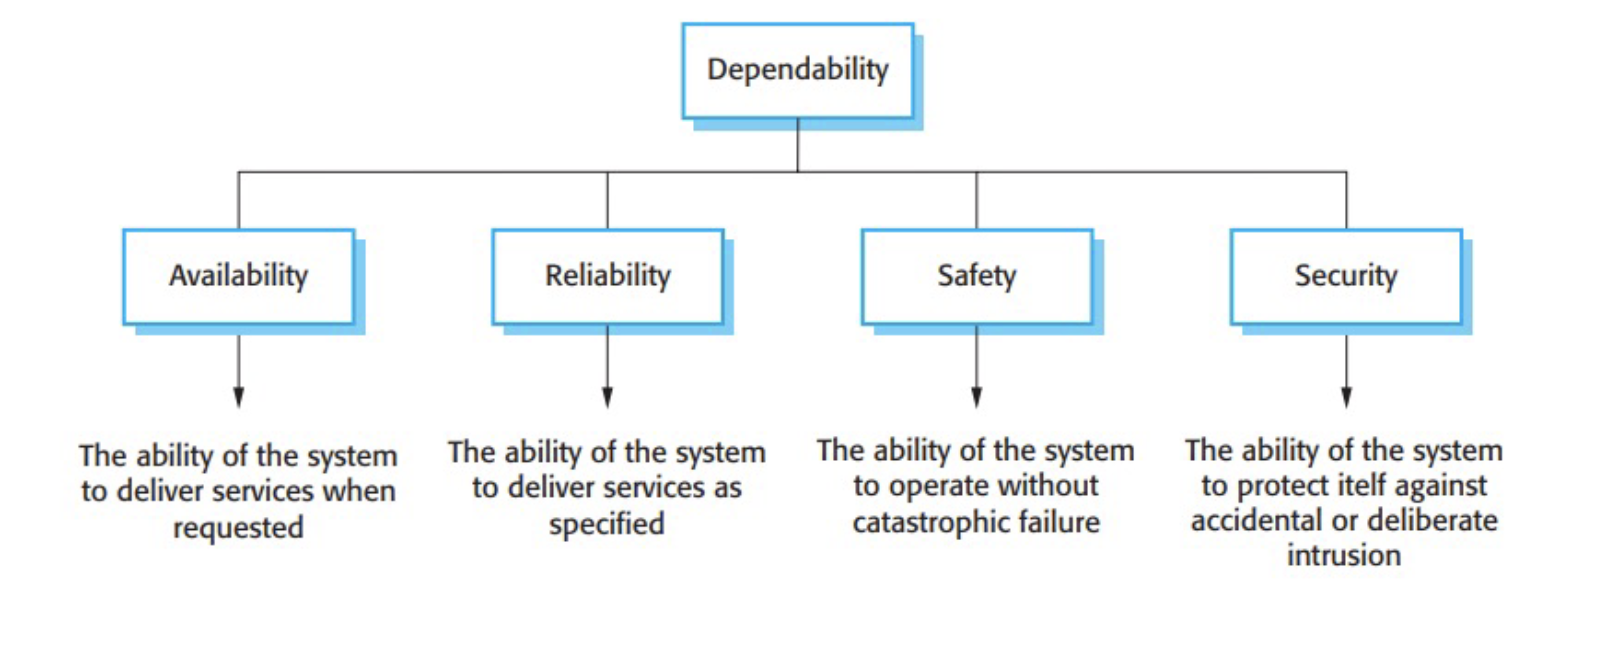
\includegraphics[width=12cm]{assets/dependability.png}
    \caption{Diagram showing the different parts of dependability [32].}
    \label{fig:dependability}
  \end{figure}

  \subsection{Reliability and fault tolerance}
  Availability and reliability are closely linked. The image below describes the difference.
  \begin{figure}[H]
    \centering
    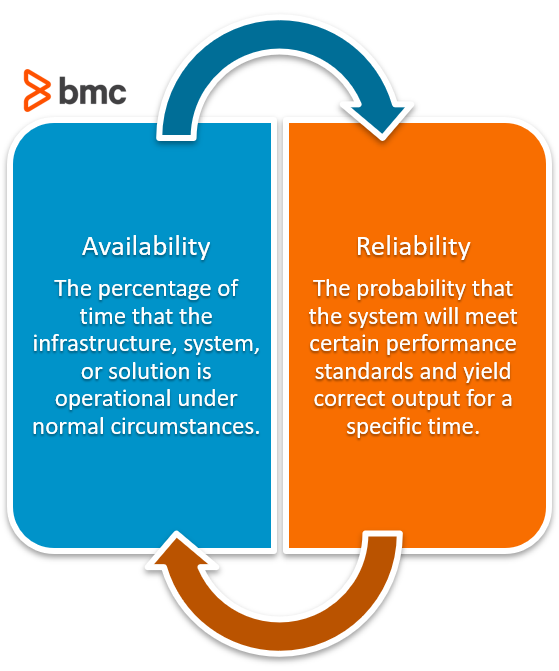
\includegraphics[width=5cm]{assets/avail-reliab.png}
    \caption{Diagram showing the difference between availability and reliability [33].}
    \label{fig:availabilityVsReliability}
  \end{figure}

  \subsubsection{Metric for ACME system reliability}

  Looking at the system designed the main component is the customer web app. This needs to successfully service as many customers as is possible.
  I have chosen the metric \textbf{POFOD = 0.0001} meaning that it is acceptable for the service to be unavailable once every 1000 requests. As this is a 
  cloud-native approach ACME has no control over what AWS will do. They themselves will have systems in place to counteract this however for 99.9\% of
  requests to succeed is still high availability.

  In order to measure this requirement AWS can help us once again. AWS provides metrics for it's components. For the web app we can check the status code
  metric, if the user receives a 2** then its OK, a 4** would be a user error and a 5** would be a server error, or downtime in this case. We can 
  then use this data to check the amount of requests that have failed due to internal server errors and check it against the metric.

  \subsubsection{Fault tolerance}
  Other than third party issues there are security problems that could arise. The first thing to tackle is the code itself, the code should be written in 
  a memory safe language. Non-memory safe languages (such as C) allow programmers direct access to memory which can result in attacks such as buffer
  overflows and use-after-free attacks [34]. Such attacks can end in system failure and sometimes allow a hacker to infiltrate the system. For this 
  reason I would suggest ACME use a language like Python. Not only is it memory safe, but it's got a vibrant community and an older study showed
  that the total code written and time spent writing was the lowest out of a handful of other languages [35].

  Ian Sommerville outlines 8 steps for dependable programming guidelines [32]. I will now go through each one and give examples of how ACMEs' system can 
  handle issues in that area.

  \begin{enumerate}
    \item \textit{Limit the visibility of information in a programme} -
    \item \textit{Check all inputs for validity} -
    \item \textit{Provide a handler for all exceptions} -
    \item \textit{Minimise the use of error-prone constructs} -
    \item \textit{Provide restart capabilities} -
    \item \textit{Check array bounds} -
    \item \textit{Include timeouts when calling external components} -
    \item \textit{Name all constants that represent real-world values} -
  \end{enumerate}

  **** Talk about alarms, auto rollbacks if threshold is reached, monitoring etc. **** 
  
  \subsection{Safety and security threats}

  \subsection{Resilience}
  Might not need to do this...

\newpage
